\section{Introduction}

\paragraph{Objective}
The goal of this document is to outline the responsibilities, expectations, opportunities, and principles needed to turn a vision into reality with a group of people.

\begin{figure}[H]
	\centering
	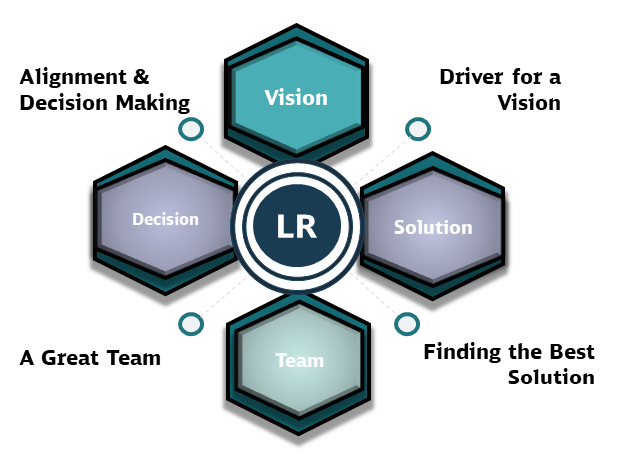
\includegraphics[scale=0.9]{attachment/chapter_OWN/Rubric_Leadership.png}
	\caption{Overview of the four responsibilities}
\end{figure}

This is not about \gls{p_LR} in the traditional sense of managing an organizational unit to ensure stable output. Instead, it focuses on creating a \gls{p_CDF} that manages expectations—both external and internal—allowing individuals to collaborate effectively to realize a shared vision based on their abilities and preferences.

This framework is a starting point, not a final solution. It should serve as a \gls{p_CDF} to help enable a group to consistently deliver the best possible solutions while moving forward with the vision. Therefore, it requires constantly scrutiny and evaluation from all perspectives.


\paragraph{Group of People or Team}
The four categories of responsibility are designed with a team in mind. However, other group dynamics such as alliances, collaborations, and social dependencies (e.g., expectations, managing membership changes, decision-making responsibilities) were also considered. The initial draft (see \ref{sec:Rubric}) failed to clearly define what constitutes a team and how the principles can be applied across different group structures. Readers are encouraged to think about how these principles apply to broader groups and not just teams. Careful thought is required when applying \gls{p_LR} in any specific context.

\section{Four Responsibilities}

\subsection{Driver for a Vision}\label{responsibility__driver}
\paragraph{Set a path: Clear, consistent, constant}

A compelling vision is essential for coherent and aligned group work. This vision acts as a guiding beacon, helping the team stay focused on a shared goal and aligning individual contributions with broader objectives. Whether the vision aligns with or sets the organization's goals, it serves as the foundation for decision-making and future strategies.

The \gls{p_LR} is to ensure that the vision remains central and influences decisions, projects, and daily discussions. While the vision doesn’t need to be detailed from the start, it should be a driving force behind the team's efforts, ideally becoming a \gls{p_CDF}.

\paragraph{Motivate Internally and Externally}
Supporting the team with external resources, information, and social support is key to achieving the vision. The \gls{p_LR} includes fostering a motivating environment both internally and externally, ensuring the team remains focused and effective.

\paragraph{The Risk: Not Having One}
A lack of clear vision poses a risk. Without clear direction, the team may struggle to coordinate efforts, and skillsets may not complement each other. If the team achieves success despite lacking a clear vision, it may be succeeding in spite of, not because of, its leadership.

\subsection{Alignment and Decision-Making} \label{responsibility__alignment}
\paragraph{Turning Plans into Action, constantly}
Turning plans into action requires constant\footnote{
	The words "constantly" and "continuously" have subtle differences. Constantly refers to something that happens repeatedly over time with possible pauses. For example, "She constantly checks her phone for messages," meaning she checks it frequently, but not without stopping. Continuously refers to something that happens without any interruption. For example, "The river flows continuously throughout the year," meaning the river flows without stopping.
}
alignment and optimal use of resources. The \gls{p_LR} is to ensure to invest constantly time and energy to be able to do that.

\paragraph{Delegation and Accountability}
Delegation is crucial for effective scaling and achieving a vision that can only be obtained through collaboration.\\

Based on the required skillset, the \gls{p_LR} is to delegate (distribute) responsibilities to the right members. This requires understanding the constraints of the group collectively and on an individual level.\\

Accountability have two parts: 
\begin{itemize}
	\item To align any divergence and ensure that the work integrates collectively. Especially in technical fields, there is a strive for elegance. This may produce singular efficiency. However, the task is to strive towards efforts that profoundly produce greater impact towards the vision. This often requires rejecting brilliant technical solutions in order to produce a greater compounded effect toward the goal.
	\item The other part is to hold the relevant delivery result against an emergent team or someone's axiomatic standard, which serves as the best guide for realizing the vision.
\end{itemize}

As usual, this is difficult from the social perspective, because you must work against the desire for group status and harmony.\\

The difference between micromanagement and effective accountability lies in giving team members the autonomy to execute tasks and find solutions while providing support and oversight as needed, instead of evaluating the solution-finding process and using one's own approach to tackling a given problem.\\

The focus is on evaluating the outcome of one's work and how it integrates with other work and the larger vision. This requires careful thought about what is really required from each part of the team and how to integrate it with the work of other team members.

\paragraph{Take the Left Decisions and Information Flow}
The term "\textit{left decisions}" refers to those crucial choices that the team or individual members either do not want or are unable to make.

Typically, these are decisions that have a significant impact and are not easily reversible. If no analytical, logical, or group consensus can be reached on these decisions, the \gls{p_LR} (primary leader's responsibility) is to make them and accept the risk of failure. However, the goal is for the group to do everything possible to find the best solution. If multiple competing solutions are presented, the team must either take on the responsibility, or if they don't, the \gls{p_LR} must assume the risk.\\

Two things are important for this process:
\begin{itemize}
	\item Arguments should be shared with as many relevant people as possible. This requires taking responsibility to ensure that individuals with reservations or critical opinions are encouraged to speak up and address their concerns clearly.
	\item If the leader determines that a final decision must be made, it is crucial to gather as much independent information from the group as possible. The leader should refrain from sharing or clarifying their position until the end. Otherwise, the information flow could become biased beforehand due to social or heuristic factors.
\end{itemize}

\paragraph{Balancing Outside Alignment with Staying True}

Analyzing and gathering information about how the outcomes of the team's work are perceived and integrated into the work of others is a critical responsibility. This alignment is essential because the team's efforts do not exist in isolation—they must fit into the larger organizational or industry-wide context. However, while external alignment is important, it must be balanced with the team’s ability to stay focused on the original vision. 

There are times when it is necessary for the team to adapt to the external environment, but there are also moments when the team should maintain the course, knowing that unique vision or long-term strategy is worth preserving. This decision is a delicate balance between reacting to the outside world and shaping it. In some cases, the team’s work may be positioned to influence the broader context or even redefine it, rather than simply responding to it.

The \gls{p_LR} is to evaluate when to prioritize external feedback and when to shield the team from distractions, ensuring that the vision remains central. This requires clear communication with the team, making sure they understand why certain adjustments are made based on outside input or why the focus remains unchanged despite external pressure. The \gls{p_LR} intails guiding the team through these decisions process.

In summary, maintaining constant alignment with external factors is important, but it must be balanced with the need to stay true to the team’s vision. The \gls{p_LR} is to make decisions on how much external influence to accept and communicate these choices effectively, keeping the team on track while also being adaptable to the larger context.

\paragraph{Balancing Focus with Contraction}

The ability to "let go of things you want to do but should not pursue" is essential.

It is crucial to avoid pursuing topics that, while valuable, should not be prioritized. \begin{center} The essence of focus lies in ignoring tasks that, while meritorious, would detract from concentrating on those that bring the most value in advancing toward the vision. \end{center}

The principle is that the team should focus on fewer topics: depth over breadth. However, the challenge also involves managing contraction. As noted in the previous paragraph, the \gls{p_LR} of balancing these two paths—focus versus contraction—is delicate. Aside from the previous paragraph, this dichotomy arises mainly from an internal well of motivation, which generates more ideas than can be realized.

Ultimately, there is the risk of focusing too narrowly on a single topic, which could either fail or become irrelevant, or conversely, not focusing enough on how it integrates with other work. Achieving this balance is key to driving the team toward meaningful, sustainable progress.

\subsection{Finding the Best Solutions} \label{responsibility__finding}
The goal is to create an environment that encourages or pushes towards finding the best solutions. This involves fostering open, solution-driven communication, promoting integrating-collaboration to find divergence, and encouraging diverse perspectives.

\paragraph{Closer to the Truth: Pushing Against a Social Equilibrium for Avoiding Conflict}

The following is a proposed hypothesis: The chance of coming closer to the "truth" requires that the group be pushed out of a social equilibrium that exists primarily to avoid individual or group conflict.

\begin{center} We sacrifice a bit of comfort for long-term success. \end{center}

The assumption is that, for our species, a stable evolutionary solution has been found: avoiding direct conflict.\footnote{
	Evolutionarily, this does not mean that this is the optimal solution. It means that our species has developed a \textbf{stable social solution} that can survive or produce positive outcomes. This explains why the term "passive-aggressive" is not something out of the ordinary under this hypothesis but rather a logical byproduct of this heuristic.
}

This equilibrium may lead to conformity and obscure differences in thought, which might otherwise be perceived as criticism or as lowering one's social standing. Moreover, identifying errors and proposing competing theories are not encouraged by this social balance. The term "truth" is not further defined here and could be explored in its own subsection. What is implied here is that we, as a group, are continuously updating our theories about the world to better align them with observations.

The primary \gls{p_LR} lies in consistently signaling safety, making it clear that the search for truth—through the critique of others' ideas—is welcomed, encouraged, and rewarded. Any perceived negative side effects of conflict-driven behavior in the pursuit of truth must be compensated for, and a stable reward system should be established.\footnote{
	This \gls{p_LR} could also be achieved by introducing a greater fear factor or by finding individuals with low fear responses.
}

Furthermore, the \gls{p_LR} also involves promoting catalytic behaviors, if necessary, to initiate a departure from the social equilibrium and in building systems that can sustain this process autonomously. However, given the nature of this assumed behavior, it is essential to recognize that even these systems require constant attention and energy to maintain.

\paragraph{Thinking Through a Concept: The Memo}

The memo-style presentation of one’s work is designed to help the author refine unfinished thoughts during the process of writing, while also providing the group with a more integrated view of the topic. This approach takes a step closer to finding the truth.\\

The memo format offers a better opportunity for the group to provide precise, critical feedback, such as identifying errors or proposing alternative solutions. While it creates additional work for the author, it reduces the risk of overlooked ideas and leverages the group's abilities to offer targeted, valuable feedback on the content.\\

This section is presented as a contrast to the modern company-style PowerPoint presentation of one’s work. PowerPoint presentations are not inherently problematic, but the issue arises when they become the sole medium—presentations without a thoroughly tested framework, theory, or actionable measures behind them.\\

The \gls{p_LR} lies in maintaining this higher standard. Because producing a memo requires more effort for most people, it also requires ongoing effort to uphold this standard. 

\paragraph{Integration Solutions}

Another guiding principle in finding the best solution is to integrate the suggested solution into the team's overall work.\\

For this, the \gls{p_LR} is straightforward but requires effort. Suggested solutions should be tested to see how well they integrate with the work of other team members. If other team members are not naturally evaluating the work, the \gls{p_LR} is to enforce this process, ensuring that the solution is tested for compatibility, alignment, and synergy with the team's efforts to achieve the shared vision. 

Otherwise, the team may not be "great", and the group could devolve into a collection of individuals working in isolation on separate tasks.

\subsection{A Great Team} \label{responsibility__great}

\paragraph{Definition}
A group of people is considered a \textbf{great team} when:
\begin{itemize}
	\item they work together in this configuration better than in any other,
	\item to achieve a particular vision within a set timeframe and with the required quality of outcomes.
\end{itemize}

A different configuration may involve removing people without replacing them, thereby making the group smaller. It could also mean changing team members to bring in higher technical skills—getting the best people. Additionally, it may involve adding people to increase output in order to achieve the vision within the given timeframe. The challenge in the latter case is to do so without slowing down progress by increasing the coordination effort.

\paragraph{Protect the Vision and the Group: Keeping the Promise}
\begin{center}
	Nobody should be surprised if they have to leave, as the group must receive the support it needs.
\end{center}
The promise is that if you join our group, you are striving to:
\begin{itemize}
	\item \textit{align your work with the overall vision},
	\item \textit{work towards aligning with your coworkers' efforts}, and
	\item \textit{evaluate your own skills} to ensure they are the right fit to serve the team's goals.
\end{itemize}
The leadership's responsibility is to clearly communicate these expectations to members when they join the group.\\

If this promise cannot be kept, then the socially difficult \gls{p_LR} (primary leadership responsibility) is to ensure:\footnote{
	This process is difficult for the team, the leader, and the individual in question because no one wants to see someone suffer, even if it's short-term. No one wants to confront a fellow team member, and no one wants to be excluded. This makes it hard for everyone to move beyond merely thinking about it and actually acting on it.
}
\begin{itemize}
	\item The individual must \textbf{leave the team}, or
	\item This person must \textbf{be kept away} from the team to protect its resources, focus, and commitment.
\end{itemize}
The team itself can also be a valuable source of insight during the evaluation process.\\

The leader is responsible for guiding the team safely through this information-gathering process. "Safely" because without practice, this is a difficult social situation to manage. The advantage is that it allows everyone to understand what it takes to be part of the team, reflect on themselves, and address issues before any action needs to be taken.\\

If the leader observes or deduces from the group's behavior that an individual cannot or will not keep their promise, then this hypothesis should be tested by guiding the group to evaluate the situation:
\begin{itemize}
	\item Is the person keeping their promise in terms of skills, feedback culture, and alignment?
	\item Or is this person causing others to falter?
\end{itemize}
If the group identifies a trade-off or offset, the hypothesis may be rejected, or the leader may \textit{disagree and commit} to the group's analysis until new information arises.\\

However, if the information collected indicates that the individual \textit{should leave} or that the team \textit{must be protected}, the \gls{p_LR} is to act on this evaluation.

\paragraph{Can't Do It, Must Say It}
If the \gls{p_LR} can be fulfilled, the responsibility lies in evaluating the set vision and goals. If the realization is that these goals can't be achieved with the current configuration, this must be communicated to the team.\\

The reason for this is that individuals joined the group to realize the vision, achieve the goals, or work in a great team. The \gls{p_LR} is to inform them so they can either recommit to the vision, accept the new goals, or leave if they prefer.

\paragraph{Scale}
The initial \gls{p_LR} lies in assessing whether scaling is necessary. This also includes having the ability to act on this assessment by securing the necessary capital investment to fund the scaling process.\\

When adding new members, leadership must carefully balance the benefits of increased capacity against the risk of greater complexity in communication and collaboration. Additional members can help meet tight deadlines, fill skill gaps, or distribute workloads more evenly. However, the inclusion of new people should not dilute the team's focus or reduce the quality of the output. The key is to integrate new members in a way that enhances productivity without overwhelming the existing team with added coordination and management tasks.

Thus, there is a continuous \gls{p_LR} to constantly evaluate whether scaling, shrinking, or other changes are required, and to act upon those findings accordingly.
